%%
%% Copyright 2007, 2008, 2009 Elsevier Ltd
%%
%% This file is part of the 'Elsarticle Bundle'.
%% ---------------------------------------------
%%
%% It may be distributed under the conditions of the LaTeX Project Public
%% License, either version 1.2 of this license or (at your option) any
%% later version.  The latest version of this license is in
%%    http://www.latex-project.org/lppl.txt
%% and version 1.2 or later is part of all distributions of LaTeX
%% version 1999/12/01 or later.
%%
%% The list of all files belonging to the 'Elsarticle Bundle' is
%% given in the file `manifest.txt'.
%%

%% Template article for Elsevier's document class `elsarticle'
%% with numbered style bibliographic references
%% SP 2008/03/01
%%
%%
%%
%% $Id: elsarticle-template-num.tex 4 2009-10-24 08:22:58Z rishi $
%%
%%
\documentclass[final,3p]{elsarticle}

%% Use the option review to obtain double line spacing
%% \documentclass[preprint,review,12pt]{elsarticle}

%% Use the options 1p,twocolumn; 3p; 3p,twocolumn; 5p; or 5p,twocolumn
%% for a journal layout:
%% \documentclass[final,1p,times]{elsarticle}
%% \documentclass[final,1p,times,twocolumn]{elsarticle}
%% \documentclass[final,3p,times]{elsarticle}
%% \documentclass[final,3p,times,twocolumn]{elsarticle}
%% \documentclass[final,5p,times]{elsarticle}
%% \documentclass[final,5p,times,twocolumn]{elsarticle}

\usepackage{hyperref}
\usepackage[capitalize]{cleveref}

%% if you use PostScript figures in your article
%% use the graphics package for simple commands
%% \usepackage{graphics}
%% or use the graphicx package for more complicated commands
\usepackage{graphicx}
%% or use the epsfig package if you prefer to use the old commands
%% \usepackage{epsfig}

\usepackage{caption,subcaption}
\usepackage{float}

%% The amssymb package provides various useful mathematical symbols
\usepackage{amssymb}
%% The amsthm package provides extended theorem environments
%% \usepackage{amsthm}

%% The lineno packages adds line numbers. Start line numbering with
%% \begin{linenumbers}, end it with \end{linenumbers}. Or switch it on
%% for the whole article with \linenumbers after \end{frontmatter}.
%% \usepackage{lineno}
\usepackage{amsmath}
\usepackage{xfrac}

% Modify citation style.
\usepackage[numbers]{natbib}

% Packages for custom table views.
% The multirow package provides merged row cells, while booktabs allows customizing the lines.
\usepackage{multirow, booktabs}
% These packages allow colors in table.
\usepackage{color, colortbl}

% Chinese support
\usepackage{xeCJK}
\setCJKmainfont{Lantinghei TC}

%% natbib.sty is loaded by default. However, natbib options can be
%% provided with \biboptions{...} command. Following options are
%% valid:

%%   round  -  round parentheses are used (default)
%%   square -  square brackets are used   [option]
%%   curly  -  curly braces are used      {option}
%%   angle  -  angle brackets are used    <option>
%%   semicolon  -  multiple citations separated by semi-colon
%%   colon  - same as semicolon, an earlier confusion
%%   comma  -  separated by comma
%%   numbers-  selects numerical citations
%%   super  -  numerical citations as superscripts
%%   sort   -  sorts multiple citations according to order in ref. list
%%   sort&compress   -  like sort, but also compresses numerical citations
%%   compress - compresses without sorting
%%
%% \biboptions{comma,round}

% \biboptions{}

\journal{LS1012 General Biology Lab, 106-1}

% adjust the footer
\makeatletter
\def\ps@pprintTitle{%
 \let\@oddhead\@empty%
 \let\@evenhead\@oddhead
 \def\@oddfoot{\centerline{\thepage}}%
 \let\@evenfoot\@oddfoot}
\makeatother

% custom color
\definecolor{Gray}{gray}{0.9}

\begin{document}

\begin{frontmatter}

\title{作業一 Sequence Labeling}

\author{劉彥廷~B03902036}

\end{frontmatter}

%%
%% Start line numbering here if you want
%%
% \linenumbers

\section{模型敘述}	
	\subsection{資料維度}
		訓練的資料組當中(train)總共有 462 位講者,與 1716 種句子,句子的最長 frames 數為 777 個。
		藉此分類後,總共有 3696 個 frame 數長短不一的句子於訓練的資料組當中。
		
		反觀,欲送出的測試資料組(test)有 74 位講者與 342 種句子,總計有 592 個句子,最長的句子 frames 數由於訓練的資料組為 777,故這裡也將其固定在 777 未另外擴增或縮減數量。
		
	\subsection{RNN} 
	\label{sec:rnn}
		\begin{figure}[H]
			\begin{subfigure}{0.48\textwidth}
				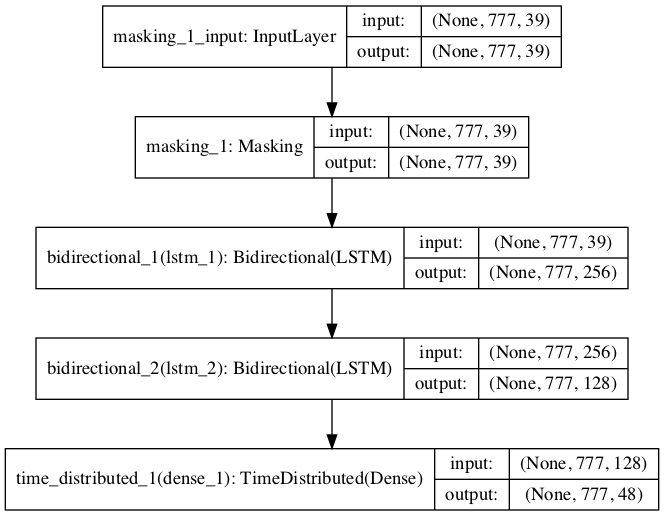
\includegraphics[width=\linewidth]{images/rnn_mfcc}
				\caption{繳交的 RNN 模型} \label{fig:rnn}
			\end{subfigure}
			\begin{subfigure}{0.48\textwidth}
				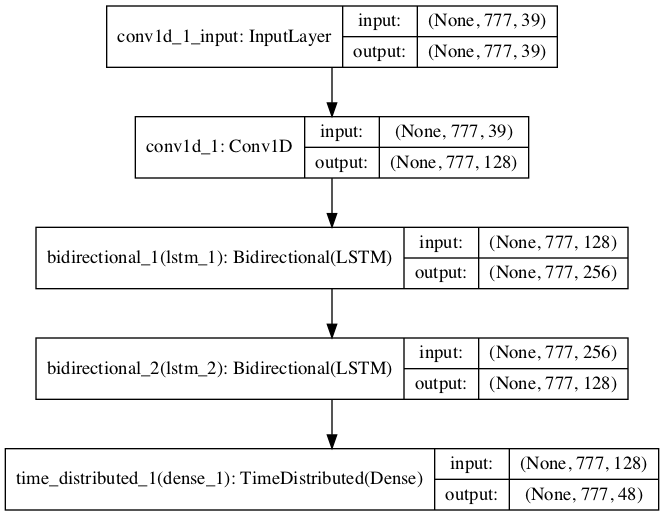
\includegraphics[width=\linewidth]{images/cnn_mfcc}
				\caption{繳交的 RNN + CNN 模型} \label{fig:cnn}
			\end{subfigure}
		\end{figure}
		Input Layer 使用了以 0 作為遮罩的 Masking Layer 讓模型忽略所有使用 0 在特徵維度進行 padding 的 frames,亦即,如果一個句子長度不足 777 個 frames,會提供各個維度特徵皆為 0 的 frames 來補足。
		
		整體設計上依照作業規格的投影片所指示的 LSTM,總計兩層 Bidirectional 的 LSTM。
		兩層各自有一組的 forward 與 backward 層,各組的單元數分別為 128 $\times$ 777 與 64 $\times$ 777。
		其中 777 這個數字乃為了滿足訓練的資料組最長的句子有 777 個 frames。
		
		Output Layer 由一層 Dense Layer 構成,裡頭的單元數恰好吻合 phones 的數量(48),activation 的方式為 softmax。
		
	\subsection{RNN + CNN}
	\label{sec:cnn}
		RNN 與 CNN 合用的模型根據作業的指示,CNN 需要放在 RNN 前端。
		由於 Keras 當中,CNN 的參數在不客製化 class 的情況下無法針對個別的特徵採用 Masking Layer 的提示,因此 Masking Layer 被拿掉了。
		剩餘的結構則維持 \cref{sec:rnn} 的架構。
		
\section{優化方式}
	\subsection{策略}
		本次作業採取的策略如下
		\begin{enumerate}
			\item 使用 MFCC 與預設的 batch size(32)以及論文 \cite{Graves_2005} 所採用的 10 個 epochs,但選用不同的模型。
			\item 在參考過 RNN 與 LSTM(在 Keras 當中的分類)的 framw-wise 準確率以後,選用 LSTM(爾後增加了 Bidirectional Wrapper)。
			\item 調整 optimizer 與初始化的 kernel(最後沒有依照論文採用的 RandomUniform),並調整 batch size 與 epochs 大小,觀察 loss 變化與 GPU 使用率和訓練時間。
			\item 反覆上述步驟。
			\item 嘗試 MFCC 與 fbank 對同樣模型的準確率差異。
			\item 嘗試在 LSTM 前面放一層 CNN 後,將 hyperparameters 多一項(卷積的 kernel size)。
		\end{enumerate}
		
		在這過程當中並沒有使用系統性的在 hyperparameter 的空間(從策略當中,可以調整的主要為 batch size、epochs 與初始化的 kernel)當中搜尋最佳值,僅人工的固定間隔取樣(例:epochs 以 10 為單位從 10 調整到 100 觀察結果)。
	
	\subsection{嘗試過的方法}
		本次作業裡頭嘗試過了
		\begin{itemize}
			\item 1 到 3 層的 GRU
			\item 1 到 3 層的 LSTM
			\item 2 層 LSTM 與 Bidirectional LSTM
			\item Bidirectional LSTM(BLSTM)使用 SGD 與 Adam 兩種不同的 optimizer
			\item BLSTM 的初始權重分別使用亂數(範圍從 -0.1 到 0.1)與全 0
			\item 1 層 CNN 放在 BLSTM 前面,並調整不同 kernel size(2 的次冪)
		\end{itemize}	
		
		最後決定了維持使用 \cref{fig:rnn} 這個模型基於跨過 baseline 且 50 個 epochs 的訓練時間約莫為 1 小時,允許我嘗試多種 hyperparameter 的設置(batch size、epochs)。
		
\section{結果}
	\subsection{fbank 與 mfcc 比較}
		filter bank 的計算緣起於聲音信號的自然特徵(由不同頻率所組成),合併上人類耳蝸的樣式;MFCC 源起於某些演算法的先天限制,而需要使用 DCT 對 filter bank 的係數做 decorrelate。
		根據 \cite{SpeechPr91:online} 的建議,如果演算法不會受到信號當中彼此高度耦合的現象影響的話,可以選用 filter bank,反之則會建議使用 MFCC。
		從實驗結果當中,在固定模型與 hyperparameters 的情況下,fbank 的結果總會比 MFCC 差了將近 50\% 的 frame-wise 準確率(79\% 與 50\% 的準確率差異)。
		考慮到我們使用了 LSTM 且使用了 Time Distributed Wrapper 讓模型可以針對時序信號自適應,信號本身隨時間的相依性可能會造成模型誤判結果(因為時間上的連續已經在模型當中被考慮了),故 MFCC 是較佳的選擇。
		
	\subsection{epochs 數}
		\begin{figure}[H]
			\centering
			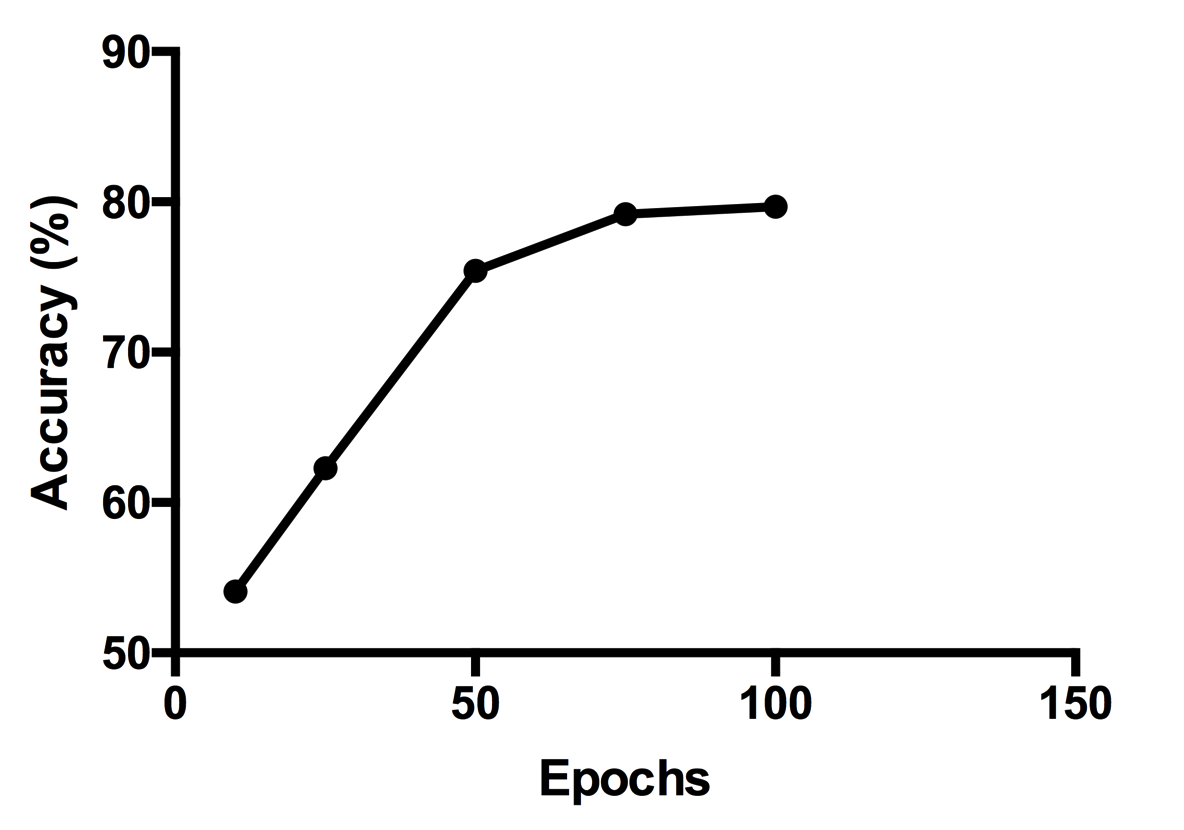
\includegraphics[width=0.4\textwidth]{images/epochs_accuracy}
			\caption{隨著 epochs 改變的 frame-wise 準確率} \label{fig:epo_acc}
		\end{figure}
		基於 CNN + BLSTM 的模型訓練至收斂($10^{-4}$)需要約莫 5 個小時的時間,這裡選擇了 \cref{sec:rnn} 的模型進行嘗試。
		儘管沒有反覆測試取得 error bar,epochs 的數量增加的確不會讓準確率無限制上升,但當時沒有考慮到 overfitting 的現象,所以沒有一併記錄下校驗組(validation set)的 loss 與 epochs 的關聯。
		
	\subsection{模型}
		礙於作業為分數導向,所以著重在不同模型對於準確率的影響,而非信號的特徵對模型不同層之間的效果。
		剛訓練完的時候,模型的 frame-wise 準確率是第一個拿到的參數,edit distance 則是事後(與 submission 後)所拿到的。
		在各自均達到收斂的情況下,BLSTM(\cref{sec:rnn})的 frame-wise 準確率大約在 79\% 而 edit distance 則為 14.1,但 CNN + RNN 的模型(\cref{sec:cnn})的 frame-wise 準確率卻下降至 32\% 附近,事後計算與 submit 後得到的 edit distance 卻依舊維持在 14 附近。
		
		比較後可以留意到 CNN + BLSTM 的模型所產出的資料(尚未刪去 consecutive phones 與前後的 sil)含有較多固定的片段,而純粹的 RNN 則容易在當中穿插不同的結果。
		這導致了 BLSTM 儘管 frame-wise 準確率偏高,但中間插入的片段導致它們無法被踢出,進而增加了 insertion 的數量。
		反觀 CNN + BLSTM,中間不確定的部分全數被抹為相同的結果,儘管 frame-wise 準確率嚴重下降,在刪減後效果依舊相似,隨機選取的句子可以發現多為 deletion 的錯誤(這需要針對整體的資料組進行 insertion、deletion 與 replacement 的統計才能進一步證實這個論點)。
		
%% References
%%
%% Following citation commands can be used in the body text:
%% Usage of \cite is as follows:
%%   \cite{key}         ==>>  [#]
%%   \cite[chap. 2]{key} ==>> [#, chap. 2]
%%

%% References with bibTeX database:
\bibliographystyle{apa}
% \bibliographystyle{elsarticle-num} 
% \bibliographystyle{elsarticle-harv}
% \bibliographystyle{elsarticle-num-names}
% \bibliographystyle{model1a-num-names}
% \bibliographystyle{model1b-num-names}
% \bibliographystyle{model1c-num-names}
% \bibliographystyle{model1-num-names}
% \bibliographystyle{model2-names}
% \bibliographystyle{model3a-num-names}
% \bibliographystyle{model3-num-names}
% \bibliographystyle{model4-names}
% \bibliographystyle{model5-names}
% \bibliographystyle{model6-num-names}

\section{參考文獻}
\bibliography{reference}

%% The Appendices part is started with the command \appendix;
%% appendix sections are then done as normal sections
% Have the appendices start with a new page.
%\newpage
%\appendix
	
\end{document}
